\documentclass[11pt,a4paper]{article}
\usepackage[T1]{fontenc}
\usepackage[utf8]{inputenc}
\usepackage{lmodern}
\usepackage{amsmath,amssymb,amsthm,mathtools,mathrsfs}
\usepackage{graphicx,float,xcolor,multicol}
\usepackage[shortlabels]{enumitem}
\usepackage[margin=27mm]{geometry}
\usepackage{microtype,needspace,placeins}
\usepackage{tikz,tikz-cd}
\usetikzlibrary{arrows.meta,calc,positioning,patterns,decorations.pathreplacing}
\usepackage[colorlinks=true,linkcolor=teal,urlcolor=teal,citecolor=teal]{hyperref}
\setlength{\parindent}{0pt}
\setlength{\parskip}{.6em}
\setcounter{secnumdepth}{0}
\allowdisplaybreaks
\raggedbottom
\providecommand{\cross}{\times}
\DeclareUnicodeCharacter{2020}{\ensuremath{\dagger}}
\DeclareMathOperator{\supp}{supp}
\DeclareMathOperator*{\esssup}{ess\,sup}
\providecommand{\chapter}{\section}
\newenvironment{tool}[2]{\subsection*{Tool #1 --- #2}}{}
\newcommand{\ToolRef}[1]{Tool #1}
\newcommand{\FigureTag}[2]{\textit{Figure #1}}
\newcommand{\Result}[1]{\subsection*{#1}}
\newcommand{\Application}[1]{\subsubsection*{Application\if\relax\detokenize{#1}\relax\else\space--- #1\fi}}
\newcommand{\ProofHeading}{\par\textit{Proof.}\space}
\newcommand{\ProofOf}[1]{\par\textit{Proof of #1.}\space}
\newcommand{\RemarkHeading}{\par\textbf{Remark.}\space}
\newcommand{\NoteHeading}{\par\textbf{Note.}\space}
\newcommand{\ExerciseHeading}{\par\textbf{Exercise.}\space}

\graphicspath{{figures/complex-analysis/}}
\begin{document}
\section*{Complex Differentiation}
% BLOG-CONTENT-BEGIN
\subsection*{Tool 5 — Epsilon-Room Method}
This is called the ``creating an $\varepsilon$ of room'' method, a very standard technique one encounters in a graduate measure theory course. Often it is not easy to prove a sharp equality or inequality. Thus, to prove something of the form $A=B$ or $A\leq B$, one tries to prove
\[
|A-B|<\varepsilon\quad(\forall\varepsilon>0)
\qquad\text{or}\qquad
A\leq B+\varepsilon\quad(\forall\varepsilon>0).
\]


From this need for an $\varepsilon$ of room, we have the following recurring, famous statement in mathematics: ``Let $\varepsilon>0$.'' This idea is a special form of routine analysis:
\[
a<b_k\ (\forall k)\Longrightarrow a\leq\inf_k b_k,
\qquad
a_k<b\ (\forall k)\Longrightarrow\sup_k a_k\leq b.
\]

\subsubsection*{Application — Complex differentiation}
Before applying Tool 5, let us look at complex differentiation.

There are two notions of differentiability in play. One occurs when $f$ is seen as a map
\[
f\colon\mathbb R^2\longrightarrow\mathbb R^2.
\]
We say that $f$ is differentiable if there is a linear map
\[
A\colon\mathbb R^2\longrightarrow\mathbb R^2
\]
such that
\[
\lim_{h\to0}\frac{|f(x+h)-f(x)-Ah|}{|h|}=0
\qquad(\forall x\in\mathbb R^2).
\]
This is a geometric notion of differentiation. There is another notion when $f$ is seen as a map
\[
f\colon\mathbb C\longrightarrow\mathbb C.
\]
We say that $f$ is complex differentiable if
\[
\lim_{h\to0}\frac{f(z+h)-f(z)}{h}
\]
exists for every $z\in\mathbb C$. This is an algebraic notion of differentiation, since it exploits the field structure of $\mathbb C$.

As metric spaces, $\mathbb C$ and $\mathbb R^2$ are homeomorphic; as vector spaces, they are isomorphic. But do these two definitions match? They ought to because $\mathbb C\cong\mathbb R^2$, and functions on $\mathbb R^2$ can be seen as functions on $\mathbb C$ and vice versa. As it turns out, a differentiable function on $\mathbb R^2$ need not be complex differentiable. Why do they not match, and how do we reconcile them? Let \(f\colon\mathbb R^2\longrightarrow\mathbb R^2\)
be differentiable, with $f'(x)=A$. Then $A$ can be realized as an $\mathbb R$-linear map from $\mathbb C$ to $\mathbb C$. But the derivative $f'(z)$ of a complex differentiable function $f\colon\mathbb C\to\mathbb C$ is a $\mathbb C$-linear map between copies of $\mathbb C$. Note that $\mathbb C$ is a field and hence a vector space over itself. Thus we demand much more from a complex differentiable function. What is it that we demand?

Write
\[
A=f'(x)=\left(\frac{\partial f}{\partial x},
\frac{\partial f}{\partial y}\right)
=
\begin{pmatrix}
\dfrac{\partial f_1}{\partial x}&\dfrac{\partial f_1}{\partial y}\\[4pt]
\dfrac{\partial f_2}{\partial x}&\dfrac{\partial f_2}{\partial y}
\end{pmatrix}.
\]
If $A$ is $\mathbb C$-linear, then
\begin{align*}
A\binom{h_1}{h_2}
&:=A(h_1+ih_2)
=(h_1+ih_2)A(1)\\
&=(h_1+ih_2)A\binom10.
\end{align*}
On the other hand, the matrix expression, viewed in $\mathbb C$, is
\begin{align*}
&\left(\frac{\partial f_1}{\partial x}h_1+
\frac{\partial f_1}{\partial y}h_2\right)
+i\left(\frac{\partial f_2}{\partial x}h_1+
\frac{\partial f_2}{\partial y}h_2\right)\\
&\qquad=(h_1+ih_2)
\left(\frac{\partial f_1}{\partial x}
+i\frac{\partial f_2}{\partial x}\right)\\
&\qquad=\left(\frac{\partial f_1}{\partial x}h_1-
\frac{\partial f_2}{\partial x}h_2\right)
+i\left(\frac{\partial f_1}{\partial x}h_2+
\frac{\partial f_2}{\partial x}h_1\right).
\end{align*}
Therefore
\[
\boxed{
\frac{\partial f_1}{\partial x}=\frac{\partial f_2}{\partial y},
\qquad
\frac{\partial f_1}{\partial y}=-\frac{\partial f_2}{\partial x}}
\]
These are precisely the Cauchy--Riemann equations. We demand that an $\mathbb R^2$-differentiable function satisfy the Cauchy--Riemann equations. Now that the condition is precise, we proceed from $\mathbb R^2$-differentiability, or Fr\'echet differentiability, to complex differentiability.

Let $f\colon\mathbb R^2\to\mathbb R^2$ be Fr\'echet differentiable and satisfy the Cauchy--Riemann equations. Then
\[
\lim_{(h_1,h_2)\to0}
\frac{\left|f(x_0+h_1,y_0+h_2)-f(x_0,y_0)-A\binom{h_1}{h_2}\right|}
{|(h_1,h_2)|}=0.
\]
Under the identifications $(x,y)\mapsto x+iy$ and $\binom xy\mapsto x+iy$, this limit is essentially
\[
\lim_{h_1+ih_2\to0}
\frac{\left|f(x_0+h_1+i(y_0+h_2))-f(x_0+iy_0)
-(h_1+ih_2)A\binom10\right|}
{|h_1+ih_2|}=0.
\]
Note that $A\binom10$, viewed in $\mathbb C$, is
\[
\frac{\partial f}{\partial x}(z_0),
\qquad z_0=x_0+iy_0.
\]
Therefore
\[
\lim_{z\to z_0}
\frac{\left|f(z)-f(z_0)-(z-z_0)\dfrac{\partial f}{\partial x}(z_0)\right|}
{|z-z_0|}=0.
\]
Since $\mathbb C$ is a field,
\[
\lim_{z\to z_0}
\left|\frac{f(z)-f(z_0)}{z-z_0}-
\frac{\partial f}{\partial x}(z_0)\right|=0.
\]
Thus
\[
\lim_{z\to z_0}\frac{f(z)-f(z_0)}{z-z_0}
=\frac{\partial f}{\partial x}(z_0)
\]
exists. Hence $f$ is complex differentiable. One can trace back, too.


\textbf{Remark.}
As in the construction of $\mathbb C$, its algebraic structure imposes rigidity. Exploiting that structure to define differentiability makes holomorphic functions far more regular than Fr\'echet differentiable functions, or even real differentiable functions.

\subsection*{Summary}
A function $f$ is holomorphic if and only if, seen as a map from $\mathbb R^2$ to $\mathbb R^2$, it is Fr\'echet differentiable and satisfies the Cauchy--Riemann equations; equivalently, its derivative, viewed as an $\mathbb R$-linear map from $\mathbb C$ to $\mathbb C$, turns out to be $\mathbb C$-linear.

\subsection*{General result: Looman--Menchoff theorem}
If $f$ is continuous on $\Omega$ and obeys the Cauchy--Riemann equations, then \(f\in H(\Omega).\)
This is just for fun.

\textbf{Remark.}
The derivative already shows that holomorphic functions are far more regular than merely Fr\'echet differentiable functions. If $f=u+iv$, then
\[
Df(z_0)=
\begin{pmatrix}
u_x&u_y\\
v_x&v_y
\end{pmatrix}.
\]
Note that the matrix is a positive scalar multiple of an orthogonal matrix, since \(u_xu_y+v_xv_y=0\)
by the Cauchy--Riemann equations. Let us see what this orthogonality leaves us with.


Let $\gamma_1(t)$ and $\gamma_2(t)$ be two curves in $\mathbb R^2$, and let them intersect at $t_0$. Suppose \(f'(\gamma_1(t_0))=f'(\gamma_2(t_0))\neq0.\)
Then
\[
\langle\gamma_1'(t_0),\gamma_2'(t_0)\rangle
=|\gamma_1'(t_0)|\,|\gamma_2'(t_0)|\cos\theta.
\]

\begin{figure}[htbp]
  \centering
  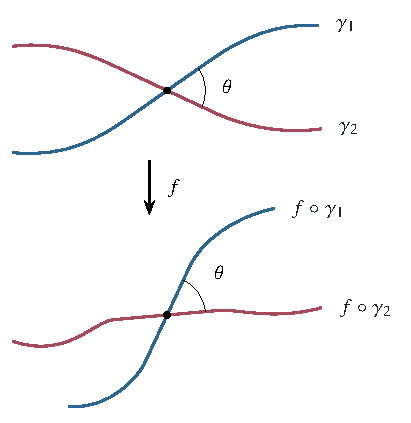
\includegraphics[width=0.64\linewidth]{note1-fig-04.pdf}

\end{figure}

Moreover,
\begin{align*}
\langle(f\circ\gamma_1)'(t_0),(f\circ\gamma_2)'(t_0)\rangle
&=\left\langle
f'(\gamma_1(t_0))\gamma_1'(t_0),
f'(\gamma_2(t_0))\gamma_2'(t_0)
\right\rangle.
\end{align*}
As $f'$ is a positive scalar multiple of an orthogonal matrix, it multiplies inner products by $|f'(\gamma_1(t_0))|^2$, so
\[
\langle(f\circ\gamma_1)'(t_0),(f\circ\gamma_2)'(t_0)\rangle
=|f'(\gamma_1(t_0))|^2\langle\gamma_1'(t_0),\gamma_2'(t_0)\rangle.
\]
Consequently,
\begin{align*}
|\gamma_1'(t_0)|\,|\gamma_2'(t_0)|\cos\theta
&=|f'(\gamma_1(t_0))\gamma_1'(t_0)|
  |f'(\gamma_2(t_0))\gamma_2'(t_0)|\cos\psi,
\end{align*}
and hence
\[
\cos\theta=\cos\psi.
\]
Assuming $\theta$ and $\psi$ are both acute, we have
\[
\boxed{\theta=\psi.}
\]

Thus $f\in H(\Omega)$ does not deform curves haphazardly: it does so in such a manner that the angle of intersection does not change. If $f\in H(\Omega)$ and $f'\neq0$ on $\Omega$, then $f$ is called a conformal map. Mind you, these maps are very rare. One result is especially useful here:

The orientation-preserving conformal automorphisms of $\widehat{\mathbb C}$ are the M\"obius transformations.
More generally, for $n\geq3$, every sufficiently smooth conformal diffeomorphism between domains in $\mathbb R^n$ is the restriction of a M\"obius transformation. In particular, the conformal automorphisms of $\mathbb R^n\cup\{\infty\}$ are the M\"obius transformations.
% BLOG-CONTENT-END
\end{document}
